\setchapterstyle{kao}
\chapter{Résultats et discussion}

% Figure caption setup
\captionsetup[figure]{format=plain,singlelinecheck=true,justification=centering}
\captionsetup[subfigure]{format=plain,singlelinecheck=true,justification=centering}

L'analyse du graphe de Software Heritage a permis de déterminer les quatre variables de recherche pour $TODO$
projets distincts dont les historique de développement sont eux aussi entièrement distincts deux à deux (aucun
projet analysé n'est un \en{fork} d'un autre).

\section{Forme et distribution des données collectées}

\begin{figure}[ht]
    \centering
    \begin{tabular}{cc}
        \begin{tabular}{ll}
 & hasContrib \\
count & 27619 \\
unique & 2 \\
top & no \\
freq & 23740 \\
\end{tabular}
 &
        \begin{tabular}{lr}
 & \textbf{recentCommitCount} \\
count & 60966.00 \\
mean & 61.79 \\
std & 408.96 \\
min & 2.00 \\
25\% & 8.00 \\
50\% & 19.00 \\
75\% & 49.00 \\
max & 36176.00 \\
\end{tabular}

        \\
        \begin{tabular}{lr}
 & \textbf{recentContributorCount} \\
count & 60966.000000 \\
mean & 3.246268 \\
std & 6.983897 \\
min & 2.000000 \\
25\% & 2.000000 \\
50\% & 2.000000 \\
75\% & 3.000000 \\
max & 688.000000 \\
\end{tabular}
 &
        \begin{tabular}{lr}
 & newContributorCount \\
count & 60966.000000 \\
mean & 0.522209 \\
std & 1.663200 \\
min & 0.000000 \\
25\% & 0.000000 \\
50\% & 0.000000 \\
75\% & 1.000000 \\
max & 130.000000 \\
\end{tabular}

    \end{tabular}

    \caption{Aperçu statistique des données collectées}
    \label{fig:data_description}
\end{figure}

Un aperçu initial des données collectées (figure~\ref{fig:data_description}) révèle quelques propriétés
intéressantes de la population étudiée. Les projets possédant des instructions de contribution ($TODO$, soit
$TODO\%$ des projets) sont significativement moins nombreux que ceux n'en possédant pas. L'écart entre la
moyenne et la médiane du nombre de \englpl{commit} récents, ainsi que sont écart type, indiquent une forte
variation de ce nombre au sein de la population étudiée, mais aussi la présence de quelques individus
extrêmes, avec un maximum à TODO \englpl{commit} récents observés dans un seul projet. Cette dernière
observation se retrouve aussi dans le nombre de \emph{contributeurs} récents, bien que de façon moins
spectaculaire. Rappelons à la vue des quantiles de cette dernière valeur que les projets ayant vu moins de
deux contributeurs distincts récents ont été exclus de l'étude (voir section
\ref{sec:constitution_echantillon} p.~\pageref{sec:constitution_echantillon}), ce qui explique que la va leur
minimale soit de deux.

\begin{figure}[ht]
    \begin{subfigure}[t]{0.3\textwidth}
        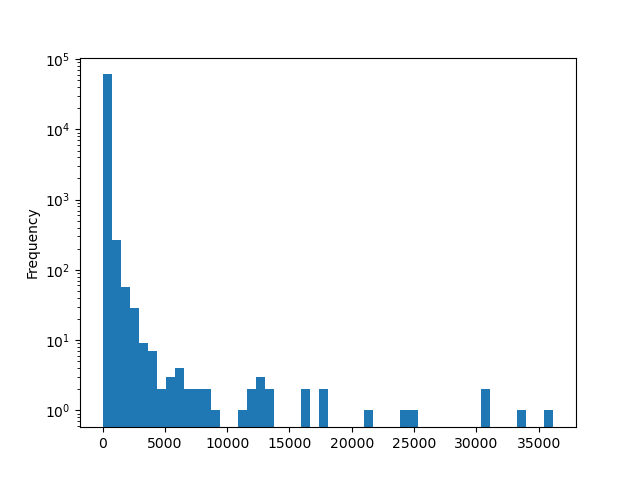
\includegraphics[width=\textwidth]{experiment/data_analysis/recentCommitCount_distribution}
        \caption{Nombre de \englpl{commit} récents\\(ordonnées logarithmiques)}
    \end{subfigure}
    \begin{subfigure}[t]{0.3\textwidth}
        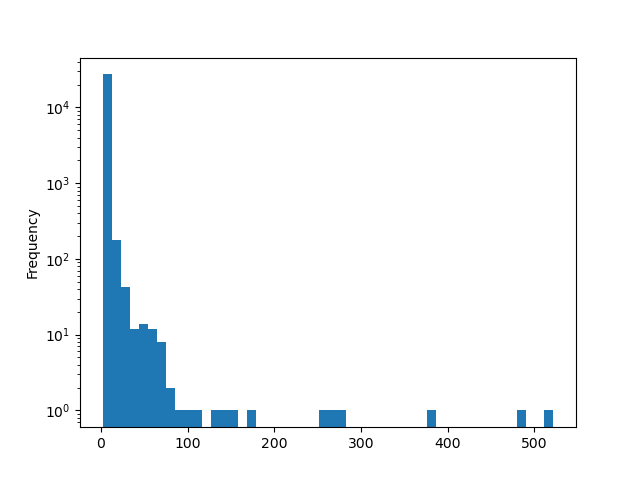
\includegraphics[width=\textwidth]{experiment/data_analysis/recentContributorCount_distribution}
        \caption{Nombre de contributeurs récents\\(ordonnées logarithmiques)}
    \end{subfigure}%
    \begin{subfigure}[t]{0.3\textwidth}
        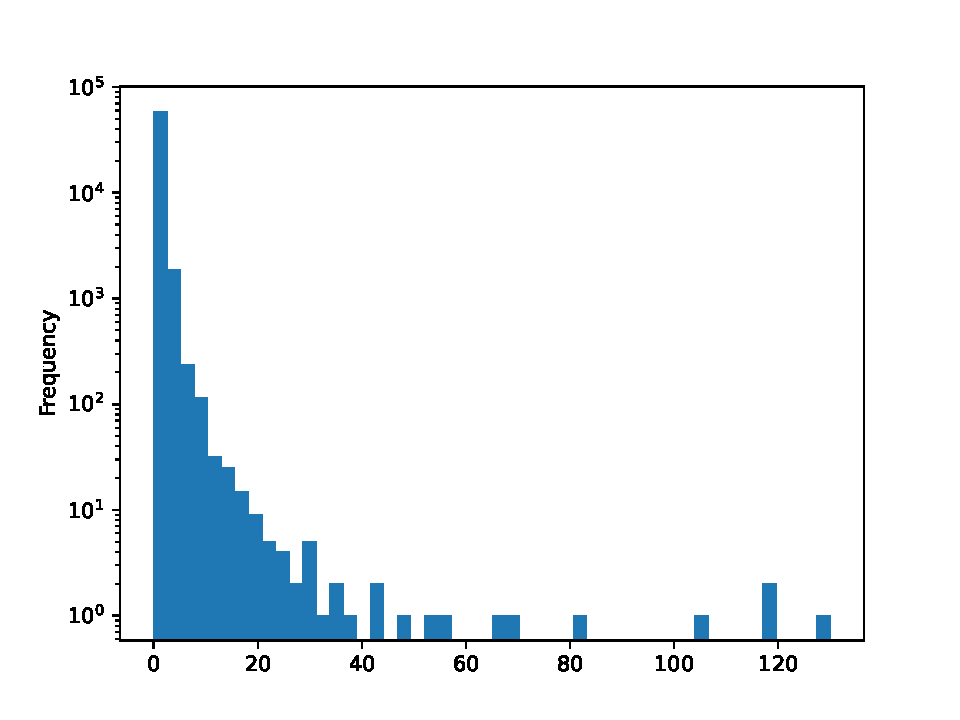
\includegraphics[width=\textwidth]{experiment/data_analysis/newContributorCount_distribution}
        \caption{Nombre de nouveaux contributeurs\\(ordonnées logarithmiques)}
    \end{subfigure}

    \caption{Distribution des individus selon chaque variable numérique}
    \label{fig:distribution}
\end{figure}

\begin{figure}[ht]
    \begin{subfigure}[t]{0.3\textwidth}
        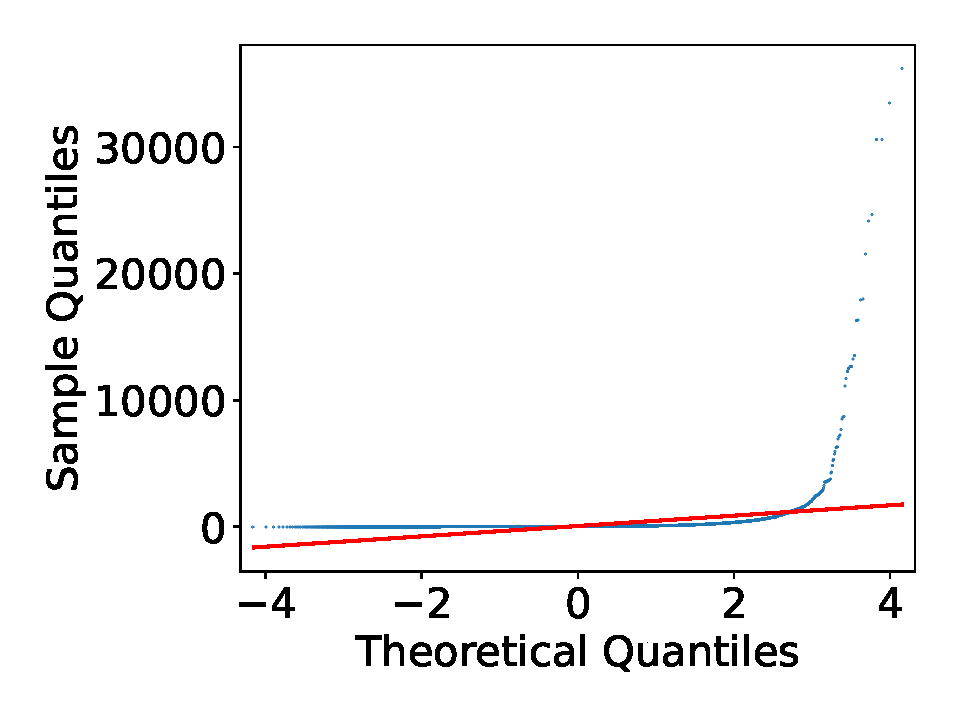
\includegraphics[width=\textwidth]{experiment/data_analysis/recentCommitCount_qqplot}
        \caption{Nombre de \englpl{commit} récents}
    \end{subfigure}
    \begin{subfigure}[t]{0.3\textwidth}
        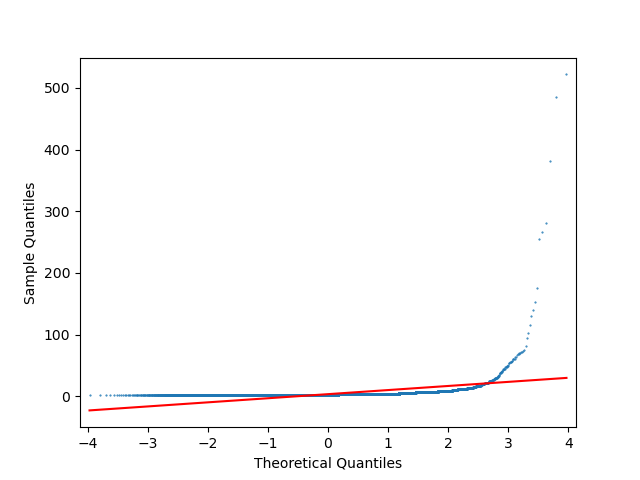
\includegraphics[width=\textwidth]{experiment/data_analysis/recentContributorCount_qqplot}
        \caption{Nombre de contributeurs récents}
    \end{subfigure}%
    \begin{subfigure}[t]{0.3\textwidth}
        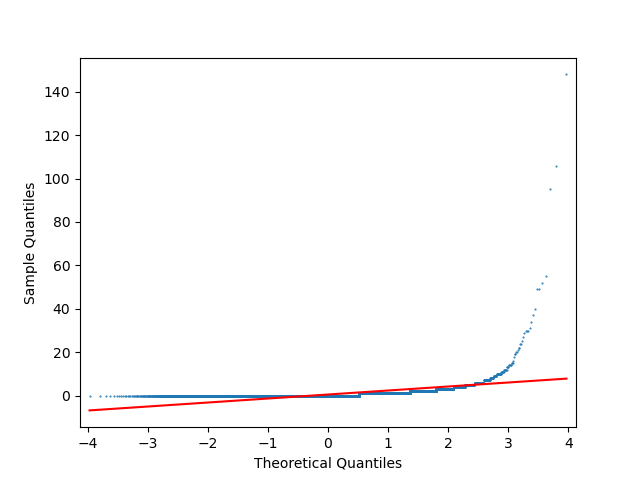
\includegraphics[width=\textwidth]{experiment/data_analysis/newContributorCount_qqplot}
        \caption{Nombre de nouveaux contributeurs}
        \label{sfig:newContributorQQplot}
    \end{subfigure}

    \caption{Diagrammes quantile-quantile pour chaque valeur numérique}
    \label{fig:qqplots}
\end{figure}

Une visualisation de la distribution de la population selon chaque variable numérique
(figure~\ref{fig:distribution}) semble donner une forme d'exponentielle décroissante pour chacune d'elles, ce
qui signifie par exemple que les projets ayant peu de nouveaux contributeurs sont les plus courants, alors que
ceux en ayant plus deviennent rapidement beaucoup plus rare à mesure que le nombre augmente. Les diagrammes
quantile-quantile (figure~\ref{fig:qqplots}) de ces variables confirment de façon un peu plus formelle que
leur distribution ne suit pas une loi normale, ce qui sera important pour l'interprétation des régressions
obtenues plus loin dans cette analyse.

\section{Lien entre la présence d'instructions de contribution et le nombre de nouveaux contributeurs}

\begin{figure}[ht]
    \begin{subfigure}[t]{0.5\textwidth}
        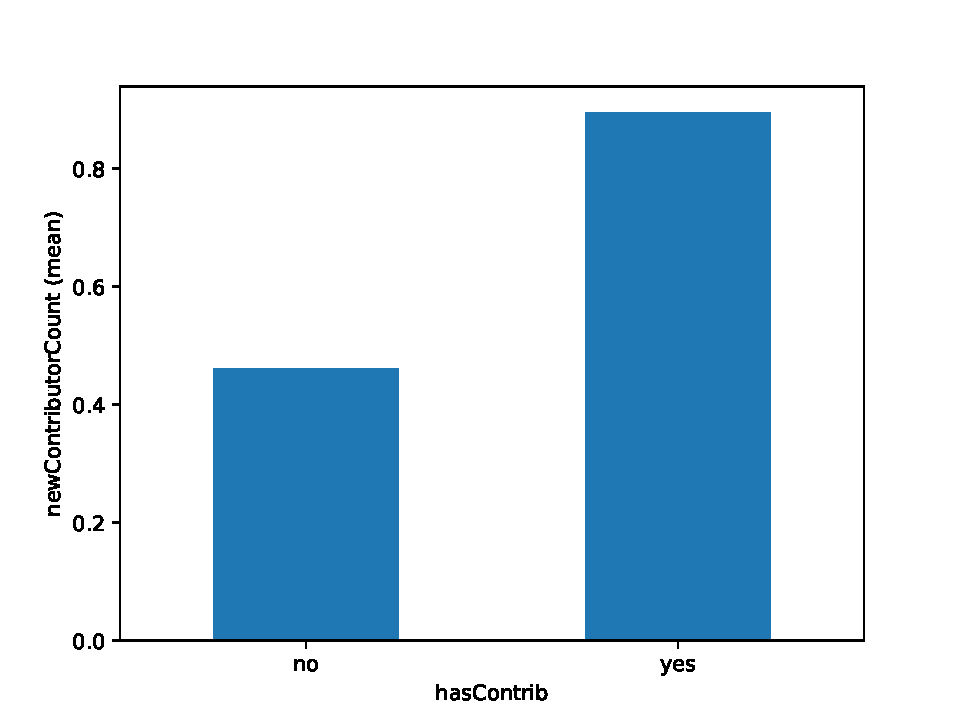
\includegraphics[width=\textwidth]{experiment/data_analysis/hasContrib_meanNewContributorCount}
        \caption{Moyenne du nombre de nouveaux contributeurs pour chaque catégorie}
    \end{subfigure}%
    \begin{subfigure}[t]{0.5\textwidth}
        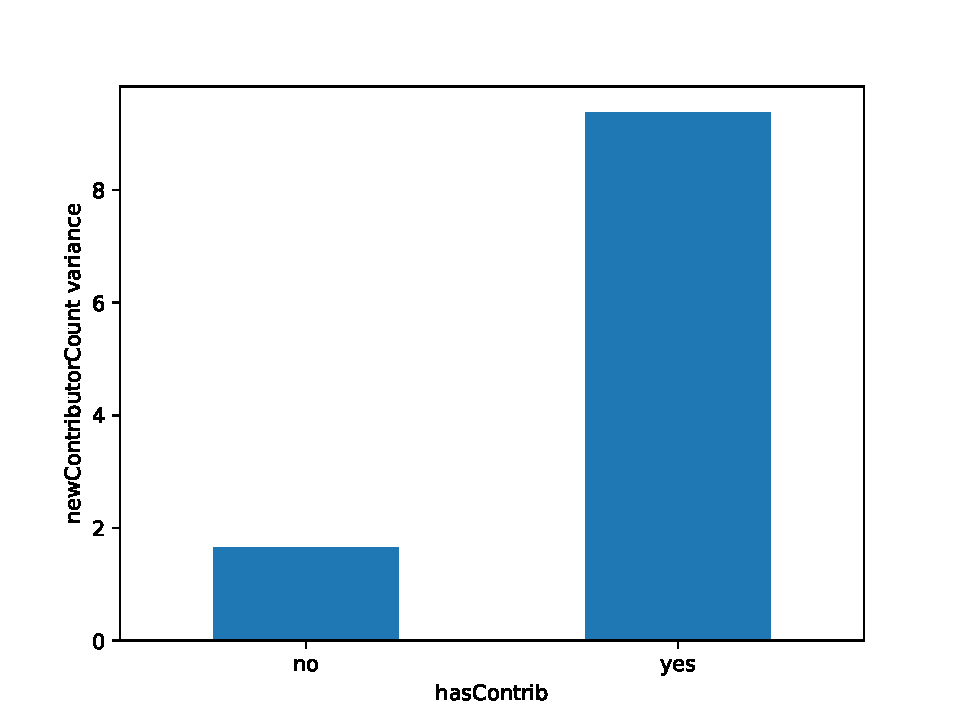
\includegraphics[width=\textwidth]{experiment/data_analysis/hasContrib_varianceNewContributorCount}
        \caption{Variance du nombre de nouveaux contributeurs pour chaque catégorie}
        \label{sfig:hasContribVariance}
    \end{subfigure}

    Mann-Whitney statistic: $U = 52115090$ ($p = 1.783731 \times 10^{-60}$, $ρ = 0.56593036$)
    \caption{Moyenne du nombre de nouveaux contributeurs pour chaque catégorie}
    \label{fig:hasContrib}
\end{figure}

La figure \ref{fig:hasContrib} montre la moyenne du nombre de nouveaux contributeurs au sein des projets
possédant des instructions de contribution d'une part, et ceux n'en possédant d'autre part.

Ces deux catégories de projets ont été comparées avec le test de Wilcoxon-Mann-Whitney. Celui-ci donne une
valeur $U = TODO$ avec une taille d'effet $ρ = TODO$, ce qui signifie en langage courant que si l'on choisi au
hasard un projet $A$ possédant des instructions de contribution et un projet $B$ n'en possédant pas, il y a
environ $TODO\%$ de chances que le projet $A$ ait vu un plus grand nombre de nouveaux contributeurs durant la
période étudiée que le projet $B$. Le test confirme en outre avec un degré de confiance supérieur à $TODO\%$
($p < TODO$) que la distribution des valeurs au sein de ces deux catégories (projets avec instructions de
contribution ou sans) est bien différente. Le test ayant été réalisé avec l'hypothèse que les projets "avec
instructions de contribution" ont un meilleur score que les autres\footnote{hypothèse plus spécifique que la
version "\en{two-tailed}" du test}, nous pouvons formellement affirmer que cette différence est à l'avantage
des projets possédant des instructions de contribution, ce qui nous permet de valider
\hyperref[hyp:contributionguidelines]{l'hypothèse H\ref*{hyp:contributionguidelines}}.

\subsection{Discussion}

Ce résultat est cohérent avec ceux de \textcite[p.~11]{signals-2019} qui avaient déterminé que la présence
d'instructions de contribution au sein d'un projet était un signal important dans le processus de décision
d'un potentiel contributeur qui cherche un projet auquel contribuer. De futures recherches pourraient
s'intéresser à la question de savoir si ce plus grand nombre de nouveaux contributeurs \emph{ayant réussi à
contribuer} (observé dans notre étude) est dû uniquement à ce plus grand nombre de nouveaux contributeurs
\emph{essayant de contribuer} (observé par \textcite{signals-2019}), ou si la présence d'instructions de
contribution a un réel rôle dans le succès d'une tentative de contribution, en plus d'être un signal positif
attirant plus de potentiels contributeurs.

Il est tout de même important de noter que bien que le test de Wilcoxon-Mann-Whitney soit non-paramétrique et
puisse donc s'appliquer à ces données (contrairement à un test de Student nécessitant une distribution
normale, par exemple), sa robustesse diminue significativement lorsque la distribution des données ne suit pas
une loi normale \emph{et} que les groupes comparés ont une variance significativement différente
\parencite{WMW-robustness-1998}, ce qui est le cas ici (voir figures \ref{sfig:newContributorQQplot} et
\ref{sfig:hasContribVariance}). Ce point, ainsi que la petite taille d'effet obtenue, justifierait une
attention plus particulière à la préparation des données afin d'approcher une distribution normale et d'en
homogénéiser la variance, tâche qui n'a pas pu être réalisée dans cette étude faute de temps.

\section{Lien entre le nombre de contributeurs récents et le nombre de nouveaux contributeurs}

S'agissant ici de comparer deux valeurs numériques dont l'éventuelle relation n'est pas connue, le modèle
choisi est celui de la régression linéaire, visualisé en figure \ref{fig:contributorCount}.

\begin{figure}
    \centering
    \begin{subfigure}[t]{0.5\textwidth}
        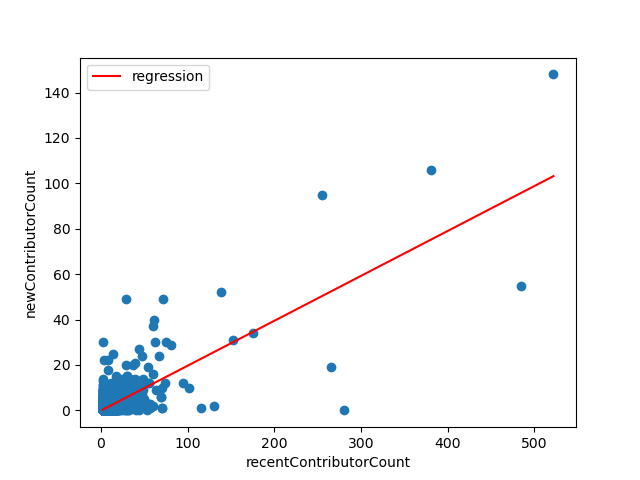
\includegraphics[width=\textwidth]{experiment/data_analysis/recentContributorCountRegression_linearScale}
        \caption{Échelle linéaire}
    \end{subfigure}%
    \begin{subfigure}[t]{0.5\textwidth}
        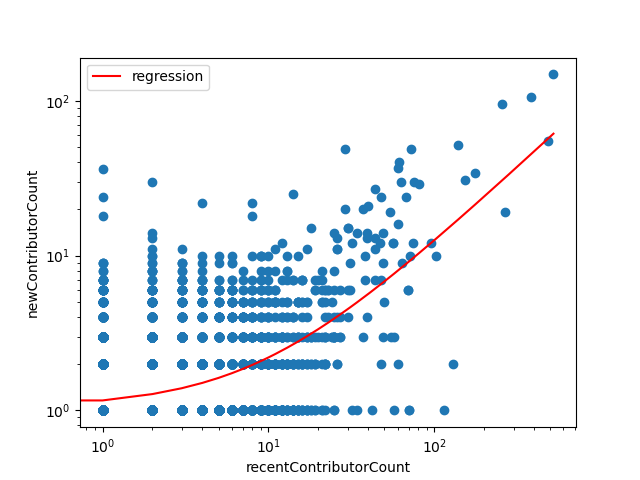
\includegraphics[width=\textwidth]{experiment/data_analysis/recentContributorCountRegression_logScale}
        \caption{Échelle logarithmique}
    \end{subfigure}

    $\mathit{newContributorCount} = \mathit{recentContributorCount} * 0.11540180 + 1.04427117$\\($r^2 = 0.28318792$)

    Test d'homoscédasticité de White : $p = 0$

    \caption{Nombre de nouveaux contributeurs en fonction du nombre de contributeurs récents uniques}
    \label{fig:contributorCount}
\end{figure}

Un premier modèle utilisant la méthode des moindres carrés ordinaires a été calculé, puis soumis à un test
d'homoscédasticité de White ayant conclu, à l'inverse, à une forte hétéroscédasticité des données de la
régression ($p = 0$). Cette hétéroscédasticité signifie que les données ont une variance fortement hétérogène
au sein du problème, ce qui implique que la méthode OLS n'est pas la plus statistiquement efficace pour
modéliser la relation entre les deux variables \parencite{GLS-2021}.

Le modèle obtenu a donc finalement été calculé par la méthode des moindres carrés généralisée\footnote{Modèle
\texttt{GLS} du paquet Python \texttt{statsmodels}:
\url{https://www.statsmodels.org/dev/generated/statsmodels.regression.linear_model.OLS.html}}, il suggère
effectivement que plus le nombre de contributeurs récents d'un projet est élevé, plus son nombre de nouveaux
contributeurs l'est aussi. Le coefficient de détermination $R^2 \approx 0.51$ du modèle indique que le nombre
de contributeur récent explique environ $51\%$ de la variation du nombre de nouveaux contributeurs, ce qui
nous permet de valider \hyperref[hyp:recentcontributorcount]{l'hypothèse H\ref*{hyp:recentcontributorcount}}
avec une taille d'effet modérée.

\subsection{Discussion}

Ce résultat est aussi cohérent avec ceux de \textcite[p.~12-13,16]{signals-2019} qui observaient que le nombre
de contributeurs uniques récents était positivement corrélé au nombre de \emph{tentatives} de contribution
faites par de nouveaux contributeurs (représenté par le nombre de \englpl{pull request}). Là aussi de futures
recherches pourraient étudier la causalité de cette relation, notre étude ne pouvant qu'affirmer que, le
nombre de contributeurs récents étant mesuré sur une période antécédente à celle sur laquelle est mesuré le
nombre de nouveaux contributeurs, cette deuxième variable ne peut pas influencer la première, du moins telles
qu'elles ont été définies ici. Il reste à déterminer si une chaîne causale lie directement ces deux variables
(si oui, laquelle) ou si elles ne sont liées que par un ancêtre causal commun (et si oui, lequel).

\section{Lien entre le nombre de \en{commits} récents et le nombre de nouveaux contributeurs}

Suivant la même approche que pour l'analyse du nombre de contributeurs récents, une première modélisation par
régression linéaire suivant la méthode des moindres carrés ordinaires a d'abord été faite. Un test
d'homoscédasticité de White a, là aussi, conclu à une forte hétéroscédasticité des données, c'est donc une
régression linéaire utilisant la méthode des moindres carrés généralisée qui a été retenue (figure
\ref{fig:commitCount}).

\begin{figure}[ht]
    \centering
    \begin{subfigure}[t]{0.5\textwidth}
        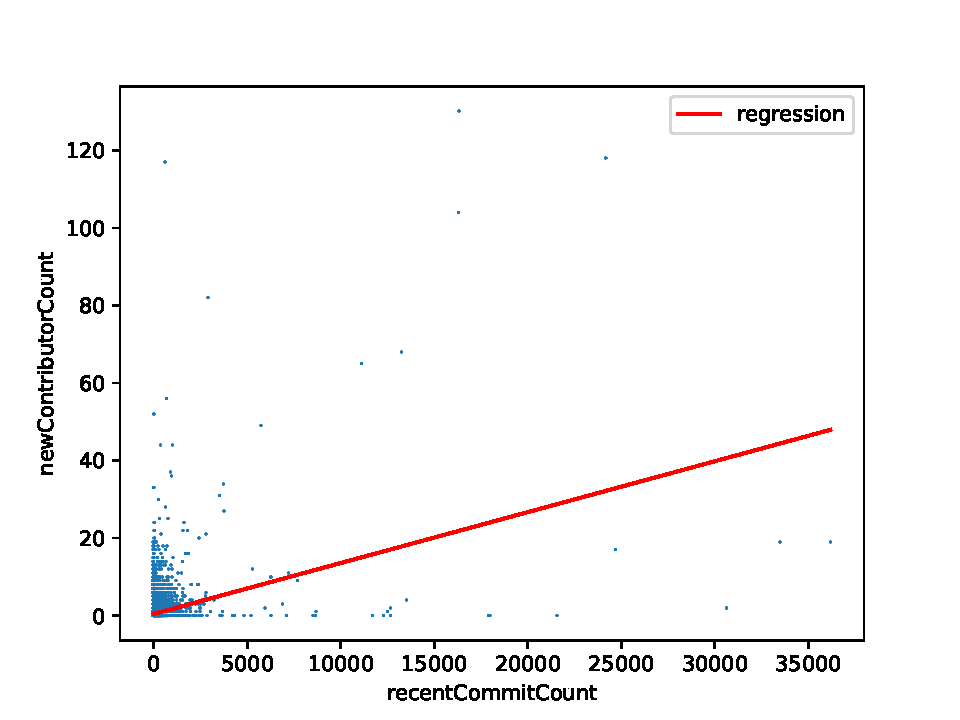
\includegraphics[width=\textwidth]{experiment/data_analysis/recentCommitCountRegression_linearScale}
        \caption{Échelle linéaire}
    \end{subfigure}%
    \begin{subfigure}[t]{0.5\textwidth}
        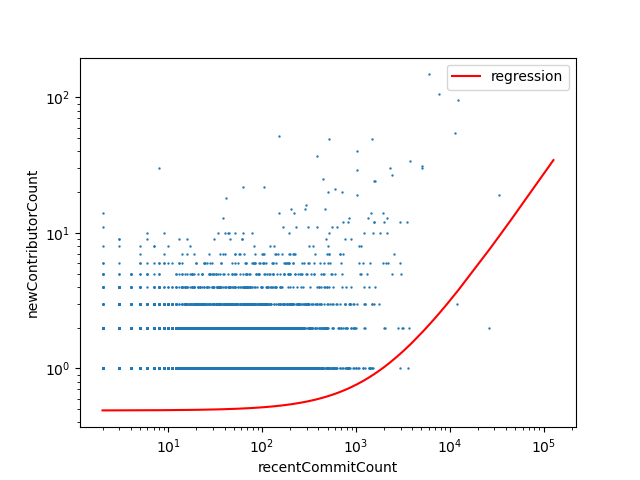
\includegraphics[width=\textwidth]{experiment/data_analysis/recentCommitCountRegression_logScale}
        \caption{Échelle logarithmique}
    \end{subfigure}

    $\mathit{newContributorCount} = \mathit{recentCommitCount} \times 0.00026672041 + 0.48979364$\\($r^2 = 0.12749825$)

    Test d'homoscédasticité de White : $p = 0$

    \caption{Nombre de nouveaux contributeurs en fonction du nombre de \englpl{commit} récents}
    \label{fig:commitCount}
\end{figure}

Le modèle suggère ici aussi une corrélation positive entre le nombre de \englpl{commit} récents d'un projet et
son nombre de nouveaux contributeurs, mais son coefficient de détermination est trop faible ($R^2 \approx
0.02$) pour considérer cette corrélation comme représentative des données du problème. Nous ne pouvons donc
conclure à une relation entre ces deux variables et devons rejeter
\hyperref[hyp:recentcommitcount]{l'hypothèse H\ref*{hyp:recentcommitcount}}.

\subsection{Discussion}

Ce résultat ne rejoint cette fois pas ceux de \textcite[p.~13,16]{signals-2019}, qui avaient là encore trouvé
une corrélation positive entre le nombre de \englpl{commit} récents d'un projets et le nombre de tentatives de
contribution faites par de nouveaux contributeurs. Cela pourrait potentiellement signifier que le nombre de
\englpl{commit} récents d'un projet est un signal que les potentiels nouveaux contributeurs utilisent \emph{à
tort} pour choisir un projet auquel essayer de contribuer. Nos résultats ne permettent pas de conclure qu'un
grand nombre de \englpl{commit} récents, bien qu'il attire les nouveaux contributeurs, est un indicateur de
l'accessibilité du projet pour ces nouveaux contributeurs.
